%%%%%%%%%%%%%%%%%%%%%%%%%%%%%%%%%%%%%%%%%%%%%%%%%%%%%%%%%%%%%%%%%%%%%%%%%%%%%%%%%%%%%%%%%%%%%%%%%%%
%%%%%%%%%%%%%%%%%%%%%%%%%%%%%%%%%%%%%%%%%%%%%%%%%%%%%%%%%%%%%%%%%%%%%%%%%%%%%%%%%%%%%%%%%%%%%%%%%%%
%%%%%%%%%%%%%%%%%%%%%%%%%%%%%%%%%%%%%%%%%%%%%%%%%%%%%%%%%%%%%%%%%%%%%%%%%%%%%%%%%%%%%%%%%%%%%%%%%%%
%%%%%%%%%%%%%%%%%%%%%%%%%%%%%%%%%%%%%%%%%%%%%%%%%%%%%%%%%%%%%%%%%%%%%%%%%%%%%%%%%%%%%%%%%%%%%%%%%%%

\chapter{Conceptos}

Para poder identificar marcadores significativos para el diagnóstico del deterioro cognitivo, 
es posible usar la técnica de 
electroencefalografía, que es usada para medir cierto tipo de actividad cerebral y que 
posiblemente esté asociada al deterioro cognitivo. 
%Una vez expuestos los conceptos pertinentes, se presenta una colección de objetos matemáticos
%(procesos estocásticos débilmente estacionarios) con los cuales se han modelado un tipo de
%actividad cerebral, y que fue comparado con mediciones de la misma.
%
%La exposición se divide en dos subsecciones marcadamente diferentes: matemáticas y 
%fisiología/psicología.
En esta sección se presenta el deterioro cognitivo en adultos mayores, con énfasis en su 
caracterización.
%La segunda subsección se centra en las herramientas estadísticas utilizadas para analizar datos 
%experimentales, entendidas no como simples \textit{técnicas} sino como objetos abstractos definidos 
%formalmente.
%
%Estas dos partes difieren no sólo en temas sino también epistemológicamente: en la primera aparecen 
%afirmaciones basadas en datos experimentales, mientras que en 
%la segunda las afirmaciones son formalmente verdaderas y demostrables en el sistema axiomático 
%usual. Respecto a estas últimas, varias de las demostraciones se presentan como apéndice junto las 
%definiciones pertinentes.

\section{Psicología}

%La demencia es un síndrome debido a la disfunción cerebral, que produce desintegración
%de la conducta en los planos intelectual y emocional, alterando significativamente la
%función social y laboral del paciente.
La \textbf{demencia} es, según el Manual diagnóstico de y estadístico de trastornos mentales 
(DSM-IV), \textit{un síndrome que consiste en el desarrollo de déficit cognoscitivos 
suficientemente graves como para interferir significativamente en las actividades laborales y 
sociales, respecto al nivel de actividad previo. 
%Aparece precedida por una enfermedad médica o el efecto de exposición prolongada a sustancias 
%tóxicas, incluso ambos.
Los sujetos con demencia tienen una baja capacidad para aprender información nueva y suelen olvidar 
lo aprendido anteriormente, siendo éste el síntoma más prominente} \cite{DCM5}.

Cuando un sujeto presenta cambios marcados en su conducta, es relativamente fácil identificar la 
demencia; caso contrario es el diagnóstico temprano de la misma, el cual es importante para un 
tratamiento adecuado que revierta o desacelere el avance de este síndrome.
%Se ha señalado que los criterios del manual DSM-IV son suficientes para este diagnóstico
%\cite{Knopman01}.

Considerando a los \textbf{adultos mayores}, entendidos como individuos de 60 años o más, conviene 
destacar que el envejecimiento es determinado por una serie de procesos moleculares, celulares, 
fisiológicos y psicológicos que conducen directamente al deterioro de funciones cognitivas, 
específicamente atención y memoria \cite{Park09}.
La funcionalidad durante esta etapa se relaciona con el estilo de vida, los factores de riesgo, el 
acceso a la educación y las acciones para el cuidado de la salud realizadas en edades más 
tempranas \cite{Sanhueza14}.

Al momento de diagnosticar deterioro cognitivo en adultos mayores, deben tenerse en cuenta el 
envejecimiento normal y la posible \textbf{pseudodemencia depresiva}, ya que presentan 
características similares. Con respecto a ésta última, definida como \textit{un trastorno del 
afecto y que produce un aparente deterioro cognitivo} \cite{DCM5}, aunque no es efectivamente un 
tipo de demencia bien puede desencadenar en demencia en ausencia de un tratamiento adecuado.

Así mismo, para realizar un diagnóstico temprano
se considerará como etapa precursora de la demencia al \textbf{deterioro cognitivo 
leve}, definido como \textit{una alteración adquirida y prolongada de 
una o varias funciones cognitivas, que no corresponde a un síndrome focal y no cumple criterios 
suficientes de gravedad para ser calificada como demencia} \cite{Robles02};
dentro del presente escrito, este síndrome será manejado como \textbf{posible deterioro 
cognitivo (PDC)} ya que el autor no tiene la autoridad ni la autorización para efectuar un 
diagnóstico clínico, y porque los síntomas en esta etapa se consideran %--afortunadamente-- 
reversibles.

%%%%%%%%%%%%%%%%%%%%%%%%%%%%%%%%%%%%%%%%%%%%%%%%%%%%%%%%%%%%%%%%%%%%%%%%%%%%%%%%%%%%%%%%%%%%%%%%%%%

\subsection{Psicometría}

En psicología los instrumentos de medición comunes son las \textbf{pruebas neuropsicológicas}, 
entendidas como muestras de alguna conducta de interés a las que se asignan puntajes para comparar 
cuantitativamente a los sujetos \cite{Ardila12}.
%
Es a través de estas herramientas que se declaran formalmente las deficiencias cognitivas o 
conductuales, así como su severidad y clasificación.

Las habilidades que se miden usando este tipo de pruebas se suelen agrupar en áreas o 
\textbf{dominios}: atención, lenguaje, cálculo, memoria y aprendizaje, percepción, motricidad, 
funciones somatosensoriales, habilidades espaciales, funciones ejecutivas, entre otros. 
La clasificación de dominios, así como la inclusión de unos u otros, suele
variar según algunos autores.
%No  existe  un  manual  de  síndromes  neuropsicológicos,  aunque  muchos  de  ellos  se incluyen 
%en el Manual Diagnóstico y Estadístico de los Trastornos Mentales (DSM-IV, 1994)  y  en  la 
%Clasificación  Internacional  de  las  Enfermedades (ICD-10,  World  Health Organization, 2007).
%
%HACER, QUIZA, UN CUADRO SOBRE LOS DOMINIOS Y SUS RELACIONES CON LAS PARTES DEL CEREBRO
%
%Varias de estos dominios tienen han sido ubicados en regiones específicas del cerebro, mientras
%que se ha reconocido que otras tienen un área de acción basta.

En el estudio realizado por Vázquez-Tagle en 2016 \cite{VazquezTagle16} se investigó el deterioro
cognitivo en el estado de Hidalgo, para lo cual se aplicó la siguiente batería de pruebas
neuropsicológicas:
\begin{itemize}
\item Estado cognoscitivo general
\begin{itemize}
\item {Evaluación Neuropsicológica (\textbf{Neuropsi})} \cite{Solis03}
\item {Mini Mental State Examination (\textbf{MMSE})} \cite{Velasco15}
\end{itemize}
\item Detectar pseudodemencia depresiva y ansiedad
\begin{itemize}
\item {Escala breve para la detección de ansiedad del anciano (\textbf{SATS})} \cite{Vargas11}
\item {Escala de Depresión Geriátrica (\textbf{GDS})} \cite{Yesavage82,Greenberg12}
\end{itemize}
\item Detectar cambios en la vida cotidiana
\begin{itemize}
\item {Escala sobre las actividades cotidianas de la vida diaria (\textbf{KATZ})} \cite{Roumec14}
\end{itemize}
\end{itemize}

%Para discriminar el PDC con respecto a la pseudodemencia depresiva, se aplicaron pruebas para el
%estado afectivo general:
%%
%\begin{itemize}
%\item {Escala breve para la detección de ansiedad del anciano (\textbf{SATS})} \cite{Vargas11}
%\item {Escala de Depresión Geriátrica (\textbf{GDS})} \cite{Yesavage82,Greenberg12}
%\end{itemize}
%
%Más aún, para poder discriminar entre el PDC y etapas más avanzadas de demencia, se aplicó un
%test de los efectos sobre la vida cotidiana:
%%
%\begin{itemize}
%\item {Escala sobre las actividades cotidianas de la vida diaria (\textbf{KATZ})} \cite{Roumec14}
%\end{itemize}

%En el conjunto de participantes que se incluyeron en el estudio 

%%%%%%%%%%%%%%%%%%%%%%%%%%%%%%%%%%%%%%%%%%%%%%%%%%%%%%%%%%%%%%%%%%%%%%%%%%%%%%%%%%%%%%%%%%%%%%%%%%%
%%%%%%%%%%%%%%%%%%%%%%%%%%%%%%%%%%%%%%%%%%%%%%%%%%%%%%%%%%%%%%%%%%%%%%%%%%%%%%%%%%%%%%%%%%%%%%%%%%%

\section{Fisiología}

El registro de la actividad eléctrica en el cerebro, referido como \textbf{electroencefalograma} 
(EEG), está tradicionalmente relacionado con la exploración de procesos mentales y sus trastornos; 
como ejemplo se puede citar que Hans Berger, reconocido como el inventor del EEG, reportó usar 
dicha técnica en 1932 para estudiar posibles cambios en un paciente con Alzheimer 
\cite{historia_eeg}.
%
%A continuación se expone el \textit{sustrato fisiológico} del EEG, es decir, el mecanismo biológico 
%que da lugar a este fenómeno.

%De manera general, el sistema nervioso central consiste en la médula espinal y el cerebro, una 
%porción altamente especializada de la primera. El cerebro se encuentra 
%%inmerso en el líquido cefalorraquídeo y 
%protegido primeramente por las meninges, varias capas de tejido conectivo irrigadas capilarmente,
%en segundo lugar por un fluido conocido como líquido encefalorraquídeo, y en tercer lugar por el 
%cráneo, un conjunto de placas óseas; en la mayor parte de la cabeza no hay tejido muscular entre
%el cráneo y la piel.
%%
%En cuanto a estructura, el cerebro se divide en tallo cerebral, cerebelo y hemisferios cerebrales 
%(ver figura \ref{lobulos}). 
%%Son los hemisferios cerebrales la estructura asociada con las 
%%llamadas \textit{funciones superiores}: atención y memoria, reconocimiento de patrones, uso del 
%%lenguaje, entre otros.
%
%\begin{figure}
%\centering
%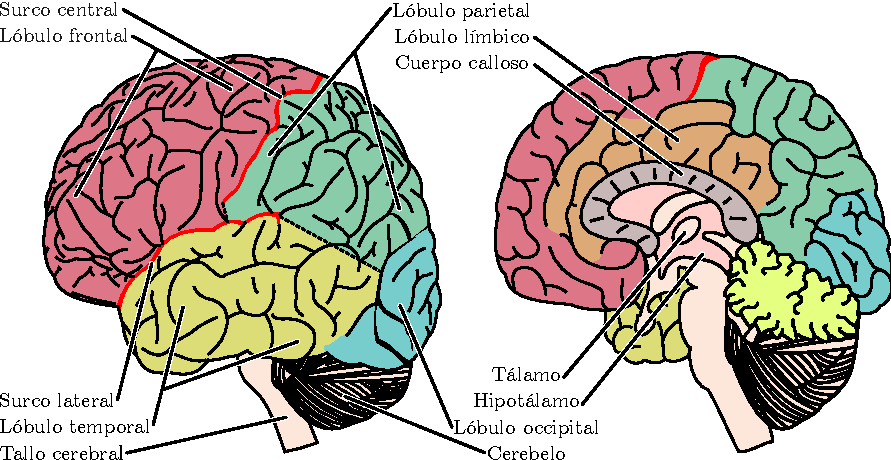
\includegraphics[width=0.7\linewidth]{./img_diagramas/cerebro_zonas_limpio.pdf} 
%\caption{División de la corteza cerebral en lóbulos}
%\label{lobulos}
%\end{figure}
%
%Los hemisferios cerebrales se estructuran en capas, de las cuales la \textbf{corteza cerebral} es
%la más externa. La corteza cerebral, o simplemente \textit{corteza}, tiene cerca de 1 cm de grosor 
%y está integrada casi exclusivamente por neuronas piramidales acomodadas 
%densamente y altamente interconectadas con neuronas en la corteza. 
%La corteza es una de las estructuras evolutivamente más recientes, siendo algunas regiones 
%exclusivas de la especie humana; se ha mostrado su papel protagónico en 
%las llamadas \textit{funciones superiores} \cite{Clark98_2}.
%% tiene cerca de 1 cm de espesor y un color grisáceo debido a que las 
%%células nerviosas en esa capa están muy densamente empaquetadas, y debido a lo cual se le conoce
%%como \textit{materia gris}.
%
%La corteza cerebral presenta numerosos pliegues estructurados en \textit{giros} (crestas) y
%\textit{surcos} (valles), los surcos más profundos son llamados \textit{fisuras}. Algunas 
%fisuras sirven como referencias anatómicas para dividir la corteza en \textbf{lóbulos}:
%la \textit{fisura lateral} define al lóbulo temporal, mientras que la \textit{fisura central} divide 
%los lóbulos frontal y parietal, como en la figura \ref{lobulos}.

%Varias de las funciones superiores han sido asociadas con regiones específicas del cerebro, por
%ejemplo, la región superior del lóbulo frontal está asociada con el procesamiento auditivo, y la
%región superior del lóbulo occipital está asociada con el procesamiento primario de imágenes;
%algunas otras funciones, como la memoria, actúan sobre múltiples estructuras 
%\cite{Clark98_2}

%%%%%%%%%%%%%%%%%%%%%%%%%%%%%%%%%%%%%%%%%%%%%%%%%%%%%%%%%%%%%%%%%%%%%%%%%%%%%%%%%%%%%%%%%%%%%%%%%%%

%\subsection{Electrofisiología}

%La parte central de la generación son las neuronas, cuyo mecanismo de transmisión a partir de
%descargas iónicas en la membrana ha sido extensamente estudiado, la descripción puede verla en
%Ermentroutt

El mecanismo base para la propoagación de campos eléctricos en las neuronas, 
depende de la capacidad de la membana celular para mantener un equilibrio estable de iones con 
el medio extracelular.
%Dicho equilibrio es contra-gradiente (implica un gasto de energía), y su estabilidad 
%potencial eléctrico a través de la membrana.
Dicho fenómeno fue ampliamente estudiado por Hodkin y Huxley, lo cual les valió el
Premio Nobel de Fisiología en 1963, y puede describirse brevemente de la siguiente manera:
cuando existe un desequilibrio puntual y súbito en la concentración extracelular de iones, se 
bombean iones a través de la mebrana para reestablecer el equilibrio en tal punto; esta acción 
genera desequilibrios secundarios en regiones vecinas de la mebrana, que a su vez activan mecanismos 
similares. Como consecuencia, la perturbación en el potencial de membrana se propaga 
a lo largo de ésta y se genera la transmisión de impulsos nerviosos en neuronas.
Un excelente referente sobre el tema es el libro por Ermentrout \cite{Ermentrout10}.

El EEG mide directamente el resultado de la transmisión de impulsos nerviosos entre neuronas de la
corteza cerebral. Contribuyen particularmente las neuronas piramidales, que se distribuyen muy densamente
formando capas, y que están altamente conectadas entre sí.

% iones a contra-gradiente a través a la 
%membrana\footnote{Debido a que la membrana celular es una permeable para moléculas pequeñas --en 
%particular iones cargados eléctricamente como sodio y potasio--, existe una presión homeostática
%que impulsa a las moléculas del sitio con mayor densidad hacia el sitio con menor densidad; los
%iones atraviesan la membrana en sicho sentido sin gasto de energía para la célula. Sin embargo,
%la membrana tiene } 
%celular. La concentración inusual, pero estable, de iones sobre la membrana celular genera un
%potencial de acción.

%(ver 
%\cite{Ermentrout10})

%\begin{figure}
%\centering
%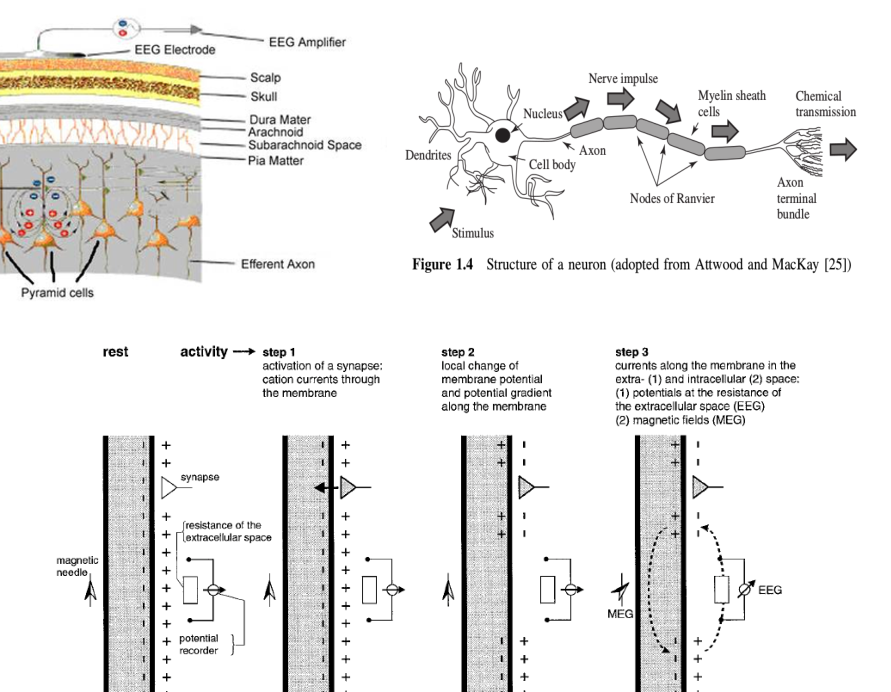
\includegraphics[width=\linewidth]{./img_diagramas/electrofisiologia.pdf} 
%\caption[Estructuras anatómicas involucradas en la generación del EEG]{Estructuras anatómicas 
%involucradas en la generación del EEG (A) Estructuras principales involucradas. (B) Neurona. 
%(C) Generación del EEG a partir de la transmisión neuronal.
%}
%\label{electro_fisio}
%\end{figure}

%%%%%%%%%%%%%%%%%%%%%%%%%%%%%%%%%%%%%%%%%%%%%%%%%%%%%%%%%%%%%%%%%%%%%%%%%%%%%%%%%%%%%%%%%%%%%%%%%%%

\subsection{Polisomnografía}

El registro de la actividad eléctrica en el cerebro se conoce como \textbf{electroencefalograma} 
(EEG); usualmente estos registros muestra una actividad oscilatoria continua y cambiante con 
frecuencia de entre 0.5 y 100 \hz; su composición está fuertemente 
relacionada con el grado de actividad cerebral mostrando, por ejemplo, diferencias claras durante 
vigilia y sueño o durante quietud y concentración \cite{Clark98_2}.
%En general la frecuencia del EEG incrementa cuando hay un altos grados de actividad cerebral, lo 
%cual se debe a que las ondas se vuelven más asíncronas, y entonces la magnitud del  potencial 
%integrado de superficie decrece (a pesar de la alta actividad cortical).

Aunque el EEG es irregular la mayor parte del tiempo, también muestra patrones relativamente organizadas 
conocidos como \textbf{ondas cerebrales}. Las ondas cerebrales más comunes y estudiadas se tipifican
en cuatro grupos según su \textit{frecuencia}: alfa, beta, gamma, delta, theta.
En la figura \ref{ritmos} se representa un arquetipo visual de cada tipo de onda.

\begin{figure}
\centering
%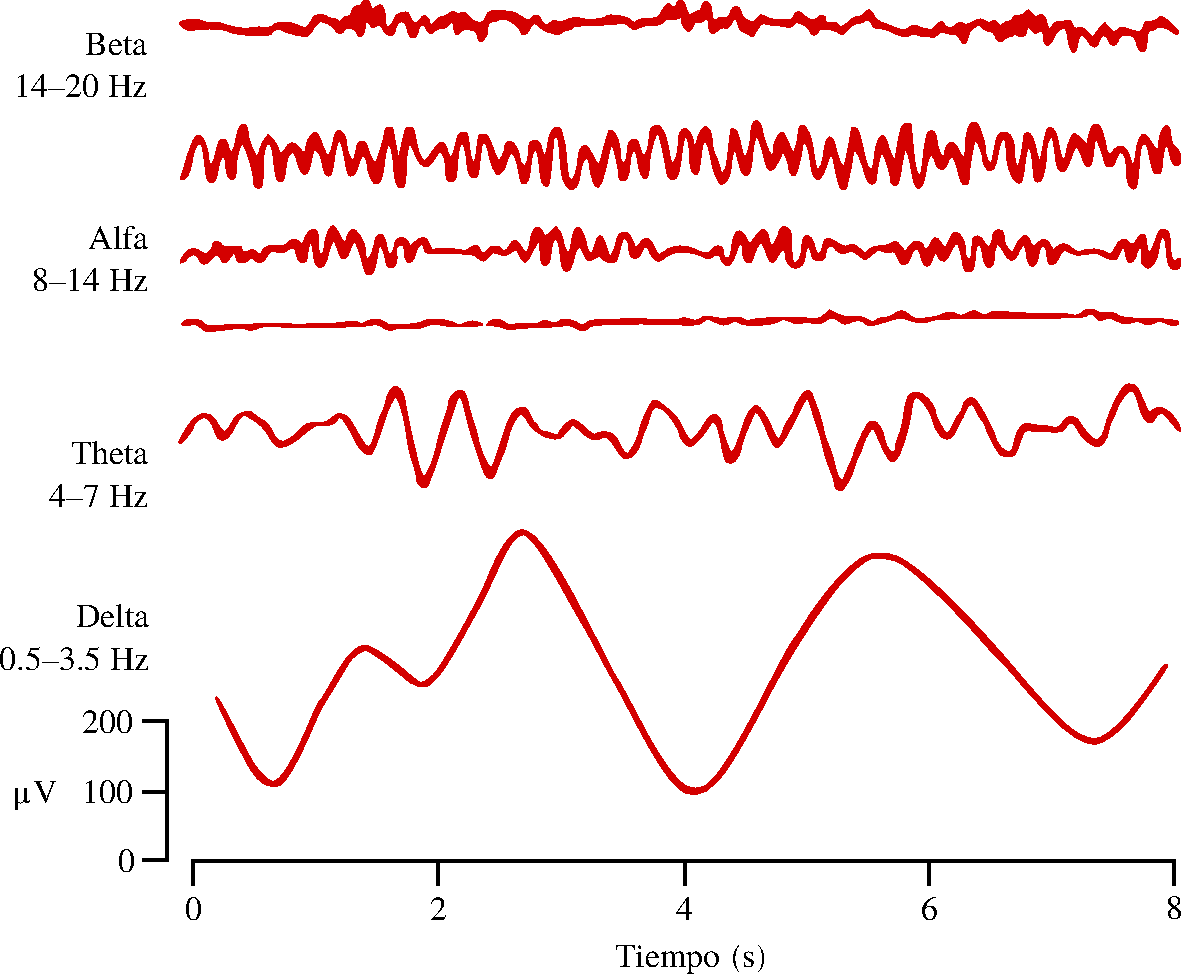
\includegraphics[width=0.55\linewidth]{./img_diagramas/ritmos_hechos.pdf} 
%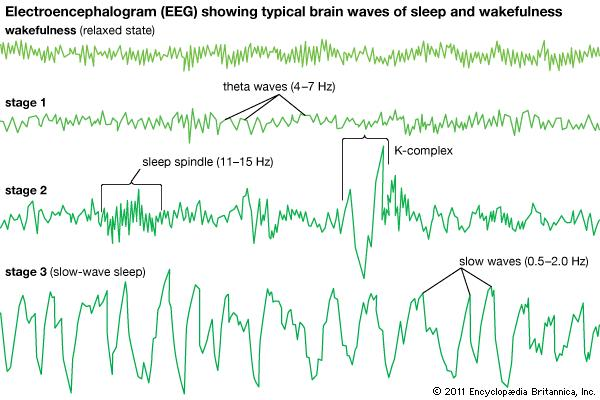
\includegraphics[width=0.9\linewidth]{./img_ejemplos/144177-004-7621DE7D.jpg} 
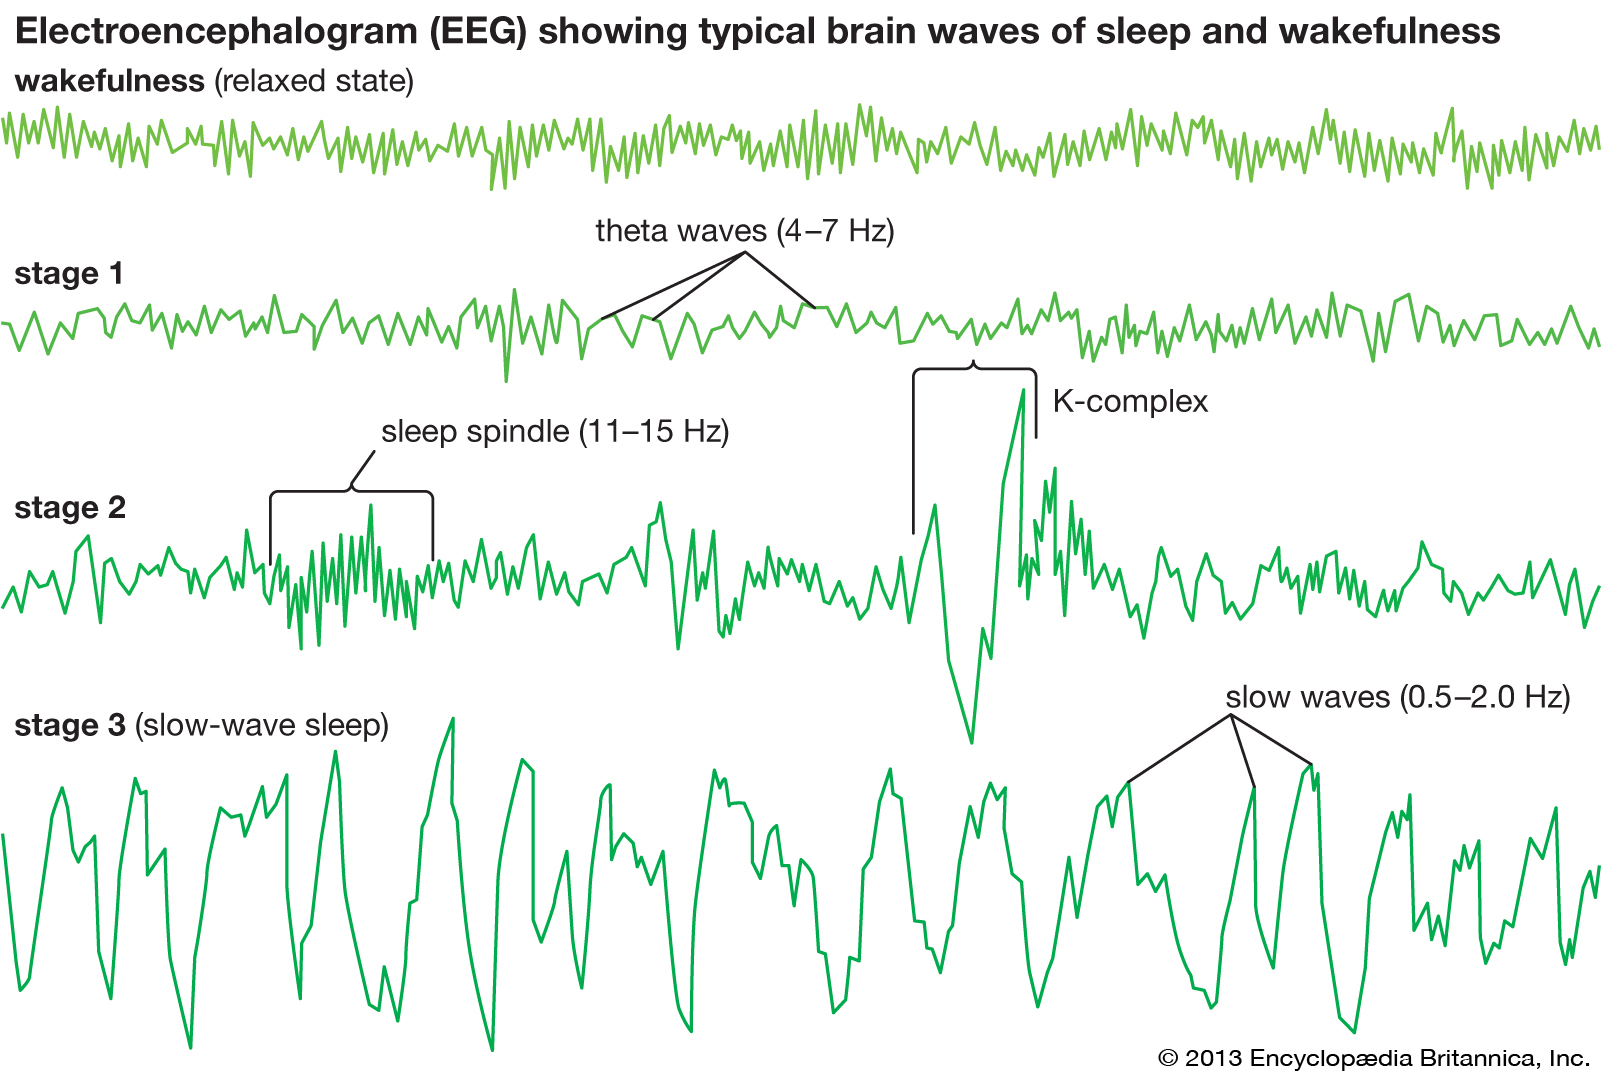
\includegraphics[width=0.8\linewidth]{./img_diagramas/ondas_britannica.jpg} 
\caption[Ejemplos de ondas cerebrales encontradas en el EEG]
{Ejemplos de ondas cerebrales encontradas en el EEG. 
Imagen tomada de Encyclop{\ae}dia Britannica, versión en línea \cite{Britannica}
%Reconstruido de \textit{EEG Signal Processing}, por S. Sanei y J. A. Chambers \cite{Sanei07} 
}
\label{ritmos}
\end{figure}

\begin{table}
\centering
\caption{Generalidades sobre ondas cerebrales}
{\small
\begin{tabular}{lclll}
\toprule
Tipo de onda
&{Frecuencia [\hz]} & {Ubicación usual} & {Condiciones usuales} \\
\midrule
{Delta} & 0.5 -- 3.5 && Síndromes focales. Sueño \\
&&& profundo en infantes \\
{Theta} & 3.5 -- 7   & P, T & Durante estrés emocional. \\
&&& En infantes \\
{Alfa}  & 7 -- 12    & F, P, O & Vigilia en reposo con \\
&& & ojos cerrados \\
{Beta}  & 12 -- 30   &P, F&      Actividad mental en\\
&&& adultos \\
{Gamma} & 30 -- 100  &&\\
&&& \\
%\midrule
%{Husos de} &&&\\
%sueño &&& \\
%{Complejo K} &&&\\
%&&& \\
\bottomrule
\end{tabular}\\
Se abrevian los lóbulos cerebrales: F=frontal, P=parietal, T=temporal, O=occipital
}
\label{tabla_ondas}
\end{table}

Para realizar el registro \textit{per se} en una forma estandarizada y comparable, se definen
arreglos llamados \textbf{montajes}, entendidos como el conjunto de (1)
los sitios donde se colocan los electrodos de registro y (2)
la manera en que los electrodos de registro están conectados entre sí.

En el trabajo de Vázquez Tagle \cite{VazquezTagle16} se usa un montaje \textit{referencial}, en el 
cual los electrodos se conectan en paralelo con un electrodo de referencia cuya actividad eléctrica 
es constante y negligible (lóbulos de las orejas, electrodos A1, A2);
los electrodos fueron colocados según el \textbf{Sistema 10--20} \cite{Jasper58,Klem99}.
%
Dicho sistema define los sitios según una cuadrícula construida respecto a distancias relativas 
entre varios puntos de referencia: el \textit{inion}, protuberancia la región posterior del cráneo, 
el \textit{nasión}, unión del hueso frontal y los huesos nasales, y el \textit{punto preauricular}, 
ubicado arriba del cartílago que protege el canal auditivo.
%llamado tragus
%y que se muestran el la figura \ref{img1020}.

%En la figura \ref{corresponde_1020} se muestran esquemáticamente las regiones de la corteza 
%cerebral que se corresponden a tales sitios (y de los cuales toman nombre); para une revisión más
%concreta de estos datos, ver .

\begin{figure}
\centering
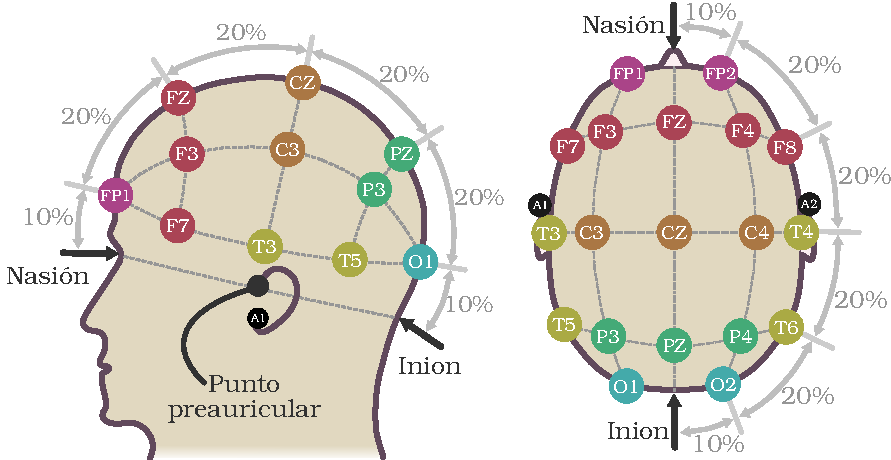
\includegraphics[width=\linewidth]{./img_diagramas/cabeza_proporcionada_color_v2.pdf} 
\caption{Colocación de electrodos según el sistema 10--20.
}
\label{img1020}
\end{figure}

%\begin{figure}
%\centering
%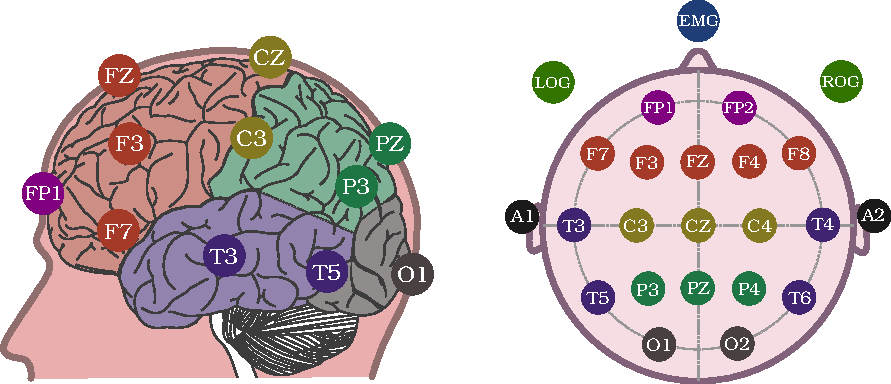
\includegraphics[width=\linewidth]{./img_diagramas/cerebro_1020_v2.pdf} 
%\caption{Correspondencia entre el montaje del Sistema 10-20 y las regiones en la corteza cerebral 
%que representan
%}
%\label{corresponde_1020}
%\end{figure}

Debido a que las neuronas en la corteza cerebral tienen orientaciones muy diversas y a que disparan 
de manera asíncrona, además de que el cerebro se encuentra cubierto por las muchas capas descritas
anteriormente, las señales captadas por los electrodos deben ser amplificadas analógicamente antes 
de ser registradas digitalmente.
A ello hay que añadir la difusión generada por las meninges, el líquido encefalorraquídeo y el 
cráneo.

%
%Cabe mencionar que ocurre una excepción importante a esta regla cuando se presenta un estímulo
%externo, lo cual provoca una respuesta simultánea; estas respuestas suelen tener una amplitud 
%relativamente alta y son referidas como \textbf{potenciales evocados}.
%
Un efecto colateral de amplificar la señal es la inclusión de \textbf{ruido}, entendido como 
señales que son registradas de manera no deseada; como ejemplo, los músculos faciales medianamente 
contraídos generan campos eléctricos con frecuencia de 100 \hz.
Este tipo de ruido \textit{persistentes} son eliminados usando un filtro que \textit{elimine} los 
componentes de frecuencia específicos.
Los ruidos de duración corta son referidos como \textbf{artefactos}; como ejemplo,
pestañear voluntariamente durante un episodio de quietud mental interrumpe las ondas alfa por cerca 
de dos segundos. El enfoque tradicional es de eliminar las porciones de registro afectadas por 
artefactos.
%La variedad de artefactos conocidos es muy basta, al grado de
%considerarse a la detección de éstos como un paso previo inevitable.

Adicionalmente al registro del EEG, el PSG incluye el registro de algunas otras \textit{variables 
fisiológicas}, como respiración, ritmo cardiaco, temperatura, entre otros. En el estudio por 
Vázquez-Tagle el registro de PSG fue complementado con registros de actividad ocular 
(\textbf{electrooculograma}, EOG) y tono muscular (\textbf{electromiograma}, EMG), según las 
recomendaciones de la AASM; la ubicación de los electrodos pertinentes es ilustrado en la
figura \ref{emg_eog}

\begin{figure}
\centering
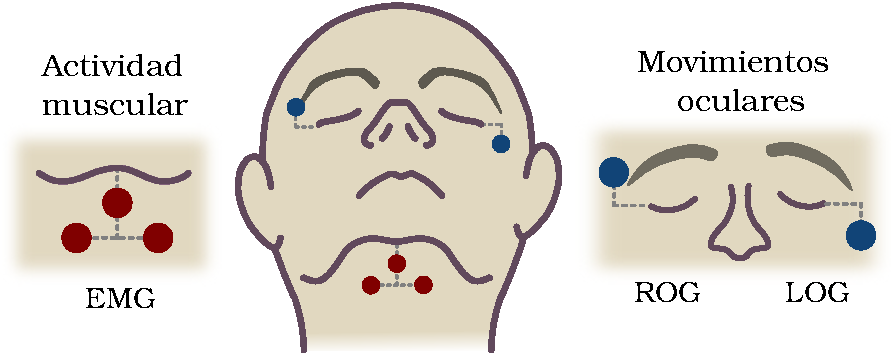
\includegraphics[width=\linewidth]
{./img_diagramas/emg_eog_v3.pdf}
\caption{Colocación de electrodos para registrar actividad ocular y tono muscular}
\label{emg_eog}
\end{figure}

Para interpretar los registros de EOG (canales LOG, ROG) se puede entender al ojo como una batería
cuyos  polos son la retina y la pupila, y que genera pequeñas variaciones en el campo eléctrico
cuando se mueve; el registro consiste en la proyección del movimiento sobre el eje que forman los
electrodos.
%
Los registros de EMG (canal EMG) admiten una interpretación más \textit{sencilla}, ya que los
músculos son activados directamente por señales eléctricas: el tono muscular es la actividad 
muscular basal, y se relaciona con la velocidad con que los músculos pueden \textit{salir} del 
reposo.

%En la figura \ref{ejemplos_mor} puede verse un ejemplo de PSG para los 22 canales en un lapso de
%10 segundos.

%%%%%%%%%%%%%%%%%%%%%%%%%%%%%%%%%%%%%%%%%%%%%%%%%%%%%%%%%%%%%%%%%%%%%%%%%%%%%%%%%%%%%%%%%%%%%%%%%%%
%%%%%%%%%%%%%%%%%%%%%%%%%%%%%%%%%%%%%%%%%%%%%%%%%%%%%%%%%%%%%%%%%%%%%%%%%%%%%%%%%%%%%%%%%%%%%%%%%%%

\subsection{Estructura del sueño}

%Se define al \textbf{sueño} como \textit{un proceso vital cíclico complejo y activo, compuesto por 
%varias fases y que posee una estructura interna característica, con diversas interrelaciones en los 
%sistemas hormonales y nerviosos};
Se entiende al sueño como un proceso vital, con una estructura característica, y que en el ser 
humano presenta las siguientes propiedades \cite{CarrilloMora}:
\begin{enumerate}
\item Disminución de conciencia y reactividad a estímulos externos
\item Fácilmente reversible, a diferencia de estados patológicos como estupor y coma
\item Inmovilidad y relajación muscular
\item Periodicidad típica circadiana (diaria)
\item Los individuos adquieren una postura estereotipada
\item La privación induce alteraciones conductuales y 
fisiológicas, además de que genera una \textit{deuda} acumulativa
\end{enumerate}

La duración del sueño es determinada en gran parte por la edad; el recién nacido duerme entre 14 y 
18 horas, el lactante entre 12 y 14 horas, el niño en etapa escolar entre 11 y 12 horas y en la 
edad adulta, la mayoría duerme entre 7 y 8 horas por noche \cite{Contreras13}.
Paralelemante el sueño no es un proceso homogéneo, sino que tiene una estructura 
por etapas con rasgos electroencefalográficos y fisiológicos distintivos.

%Según la tradición iniciada por Aserinsky y Kleitman en 1953, la clasificación del sueño
Para su estudio, el sueño se divide en dos etapas: N y R.
La \textbf{fase N}, se caracteriza por movimientos oculares lentos, tono 
muscular que decrece constantemente, actividad cerebral que recuerda al reposo, y la presencia de
husos de sueño y complejos K; en base a ello se divide en las sub-fases N1, N2, N3.
%
%El sueño fuera de la etapa MOR es referido como no-MOR (NMOR, fase N), y es dividido en etapas 
%según la 'profundidad' del sueño, entendida en términos de la actividad cerebral registrada.
%En el sueño profundo se observan ondas delta muy irregulares, y junto con ellas ocurren trenes 
%cortos de ondas, parecidas a las alfa, y que son referidas como \textit{husos de sueño}. 
%El ritmo alfa y los husos de sueño están sincronizados en el sueño y la somnolencia, en 
%contraste con la actividad irregular, desincronizada y de bajo voltaje registrada en estado de 
%alerta.

Durante la \textbf{fase R} el tono muscular disminuye (excepto para los músculos respiratorios 
y los esfínteres), la frecuencia cardiaca y respiratoria se vuelve irregular, y el sujeto exhibe 
movimientos oculares rápidos (MOR); en base a lo cual la fase R es conocida 
como \textbf{sueño MOR}.
En el EEG, aparecen ondas rápidas de bajo voltaje, irregulares, y que recuerdan la actividad 
durante el estado de alerta; estos patrones no interrumpen el sueño sino que, contrariamente,
incrementan el umbral para estímulos externos, motivo por el cual esta fase también es referida como 
\textbf{sueño paradójico}.
%
Cabe mencionar que durante el sueño MOR se producen la mayoría de las ensoñaciones (referidas 
coloquialmente como \textit{sueños}), y que la mayoría de los pacientes que despiertan durante esta 
fase suelen recordar vívidamente el contenido de sus ensoñaciones 
\cite{Rosales14}.

\begin{table}
\caption[Criterios para la clasificación de etapas de sueño]
{Criterios para la clasificación de etapas de sueño según la AASM}
\centering
{\small
\begin{tabular}{lllll}
\toprule
&&   & Movimientos & Tono \\
\multicolumn{2}{l}{Etapa}& Características del EEG & oculares & muscular \\
\midrule
Vigilia & W  & {Ritmo alfa} en $>50$\% de la época en   & No & Alto \\
        &    & la región occipital                &    &      \\
NMOR 1  & N1 & Cambio de alfa por AABFM, atenuación & Lentos & $<$W     \\
        &    & del ritmo dominante. Ondas agudas   &    &      \\
NMOR 2  & N2 & Husos de sueño y complejos K en la    & No & $<$W, $>$R     \\
        &    & primera mitad de la época. AABFM &    &     \\
NMOR 3  & N3 & {Ondas lentas} (0.5--2 \hz, $>75$ \mv) en& No & $<$N2, $\approx$R \\
        &    & $>20$\% de la época. Husos de sueño       &&      \\
MOR     & R  & Actividad baja amplitud y frecuencias & MOR's & Bajo  \\
        &    & mixtas. Ondas 'saw-tooth'             &       &       \\
\bottomrule
\multicolumn{4}{l}{Se abrevia AABFM=Actividad de Amplitud Baja y Frecuencias Mixtas}
\end{tabular}\\
}
\end{table}

\begin{figure}
\centering
\includegraphics[width=\linewidth]
%{./img_ejemplos/MJNN__epoca.pdf}
{./img_ejemplos/MJNN_epoca_stam.pdf}
\caption[Registro de polisomnograma durante sueño MOR]
{Registro de polisomnograma durante sueño MOR. Marca de calibración: vertical, 10 \mv,
horizontal, 1 segundo}
\label{ejemplos_mor}
\end{figure}

%En otras palabras, es fisiológico que el número de horas dormidas vaya disminuyendo progresivamente 
%a lo largo de la vida, pudiendo existir una diferencia de hasta 16 horas como promedio entre la 
%niñez y la edad adulta. En los ancianos, el número de horas de diferencia entre las horas de sueño 
%propias v/s las horas de sueño de la niñez, es aún mayor

%Un adulto joven pasa aproximadamente entre 70--100 minutos en el sueño NMOR para después entrar 
%al sueño MOR, el cual puede durar entre 5--30 min; este ciclo se repite cada hora y media.
%En los ancianos se va fragmentando el sueño nocturno con frecuentes episodios de despertar, se 
%reduce mucho el porcentaje de sueño en fase 4, pero se mantiene constante el porcentaje de 
%sueño MOR. Adicionalmente, muchos adultos mayores dormitan durante el día varias siestas cortas 
%\cite{CarrilloMora}.

%textwidth: \printinunitsof{cm}\prntlen{\textwidth}
%
%linewidth: \printinunitsof{cm}\prntlen{\linewidth}

%%%%%%%%%%%%%%%%%%%%%%%%%%%%%%%%%%%%%%%%%%%%%%%%%%%%%%%%%%%%%%%%%%%%%%%%%%%%%%%%%%%%%%%%%%%%%%%%%%%
%%%%%%%%%%%%%%%%%%%%%%%%%%%%%%%%%%%%%%%%%%%%%%%%%%%%%%%%%%%%%%%%%%%%%%%%%%%%%%%%%%%%%%%%%%%%%%%%%%%
%%%%%%%%%%%%%%%%%%%%%%%%%%%%%%%%%%%%%%%%%%%%%%%%%%%%%%%%%%%%%%%%%%%%%%%%%%%%%%%%%%%%%%%%%%%%%%%%%%%
%%%%%%%%%%%%%%%%%%%%%%%%%%%%%%%%%%%%%%%%%%%%%%%%%%%%%%%%%%%%%%%%%%%%%%%%%%%%%%%%%%%%%%%%%%%%%%%%%%%
